\documentclass[10pt,hyperref={citecolor=blue,anchorcolor=blue,urlcolor=blue,colorlinks=true,pdfpagelabels=true},dvipsnames]{beamer}
\usetheme{IITM}

\includeonlyframes{cur}

\usepackage{mathtools}
\usepackage{accents}
\usepackage{graphicx}
\usepackage[english]{babel}
\usepackage{csquotes}
\usepackage{cancel}
\usepackage{soul}
\usepackage{appendixnumberbeamer}
\usepackage{cleveref}

\addbibresource{refs.bib}

% Custom Stuff %----------------------------------------------------------------------------------------------------------------------------------------------------------------
\newcommand{\vc}[1]{\underbar{$#1$}}
\newcommand{\mx}[1]{\mathbf{\underline{\underbar{$#1$}}}\,}

\newcommand{\uc}[1]{\underaccent{\tilde}{#1}}
\newcommand{\mc}[1]{\underaccent{\approx}{#1}}

\newcommand{\rtxt}[1]{\textcolor{red}{#1}}
\newcommand{\btxt}[1]{\textcolor{blue}{#1}}

\newcommand{\mathcolorbox}[2]{\colorbox{#1}{$\displaystyle #2$}}
\newcommand{\mhl}[1]{\colorbox{yellow}{$\displaystyle #1$}}

\renewcommand<>{\hl}[1]{\only#2{\beameroriginal{\hl}}{#1}}

\newcommand{\dd}{\mathrm{d}}

\usetikzlibrary{shadings,shapes.arrows,shapes.callouts,patterns,decorations.pathmorphing,
  decorations.markings,decorations.pathreplacing,shapes,arrows.meta}
\tikzset{
  invisible/.style={opacity=0},
  visible on/.style={alt={#1{}{invisible}}},
  alt/.code args={<#1>#2#3}{%
    \alt<#1>{\pgfkeysalso{#2}}{\pgfkeysalso{#3}} % \pgfkeysalso doesn't change the path
  },
}
\tikzset{
  highlight on/.style={alt={#1{fill=red!80!black,color=red!80!black}{fill=gray!30!white,color=gray!30!white}}},
}
\tikzset{
  nidbox/.style={fill=white, draw=red, thick, rounded corners=0.5mm, align=center}
}

\usetikzlibrary{tikzmark,calc,positioning}
\usepackage[markings,customcolors,beamer]{hf-tikz}
\hfsetfillcolor{yellow}
\hfsetbordercolor{none}

% Get rid of figure labels
\captionsetup{labelformat=empty,labelsep=none}
%----------------------------------------------------------------------------------------------------------------------------------------------------------------
\title[Abaqus4Joints]{An Abaqus-Matlab Tutorial for Jointed Systems}
\subtitle[ICJM Seminar]{International Committee on Jointed Structures Seminar Series}
\author[Balaji, N. N.]{Nidish Narayanaa Balaji}
\institute[AE, IITM]{Department of Aerospace Engineering, IIT Madras}
% ----------------------------------------------------------------------------------------------------------------------------------------------------------------

\begin{document}

\begin{frame}
  % \begin{beamercolorbox}[sep=0.3cm,ht=1.8em,wd=\paperwidth]{frametitle}
  %   \vbox{}\vskip-4ex%
  %   \strut\insertframetitle{\begin{tikzpicture}[remember picture,overlay]
  %       \node[anchor=north] at (current page.north) (A)
  %       {\includegraphics[height=1.75cm]{template/logo.png}};
  %     \end{tikzpicture}}\strut
  %   \vskip-0.5ex%				
  % \end{beamercolorbox}
  \titlepage
\end{frame}

\begin{frame}
  \frametitle{Table of Contents}
  \begin{columns}
    \centering
    \begin{column}{.5\textwidth}
      \tableofcontents{}
    \end{column}

    \begin{column}{.5\textwidth}
    \end{column}
  \end{columns}
\end{frame}

\section{Introduction}
\label{sec:introduction}

\begin{frame}
  \frametitle{The research needs of the joints community are quite unique and specific}
  \framesubtitle{\insertsectionnumber.~\insertsection}
  \begin{tikzpicture}[overlay,remember picture]
    \pgftransformshift{\pgfpointanchor{current page}{center}}

    \node[nidbox, text width=0.4\textwidth] at (-3.4521, 0.6389)
    {\textbf{The Generic Contact Problem}
      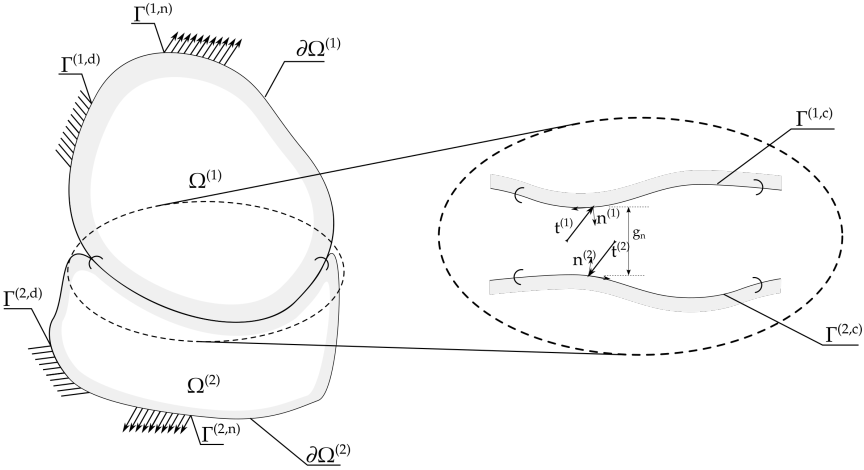
\includegraphics[width=\linewidth]{FIGS/contactprob}};

    \draw[red, very thick, rounded corners=0.5mm] (-0.4932, 2.4583) rectangle
    (6.1918, -3.0000);
    \node[align=center] at (2.8083, 2.2222) {Joints Benchmarks {\tiny
        \href{https://jointmechanics.org/index.php/Benchmarks}{(see
          jointmechanics.org)}}};
    \node[text width=0.15\textwidth] at (0.6027, 1.1528)
    {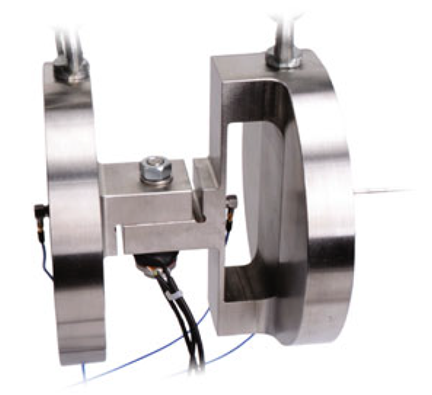
\includegraphics[width=\linewidth]{FIGS/roundres}};
    \node[text width=0.15\textwidth] at (2.4246, 1.2500)
    {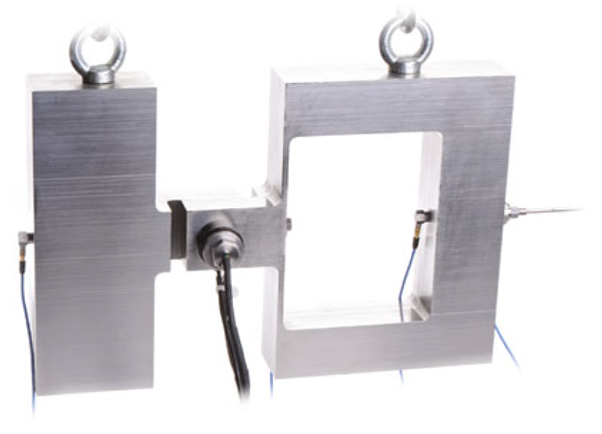
\includegraphics[width=\linewidth]{FIGS/gaulres}};
    \node[text width=0.15\textwidth] at (4.4383, 1.3055)
    {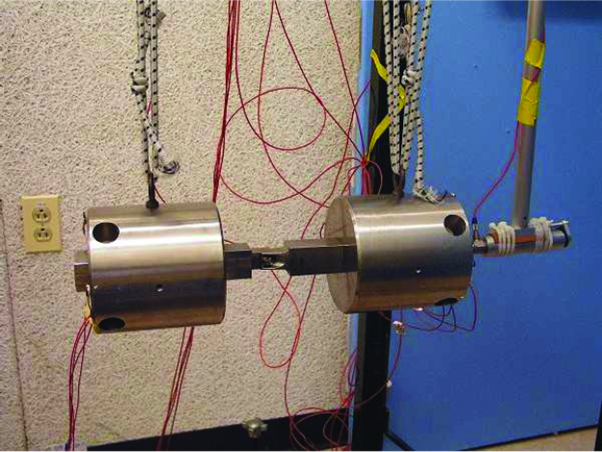
\includegraphics[width=\linewidth]{FIGS/dumbbellres}};

    \node[text width=0.4\textwidth] at (3.6987, -0.7639)
    {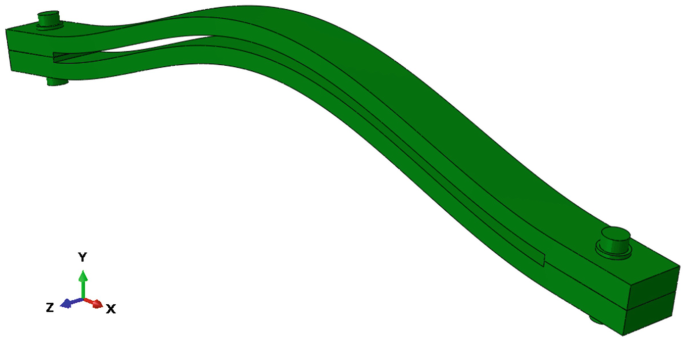
\includegraphics[width=\linewidth]{FIGS/s4bm}};
    \node[text width=0.4\textwidth] at (2.0137, -2.0138)
    {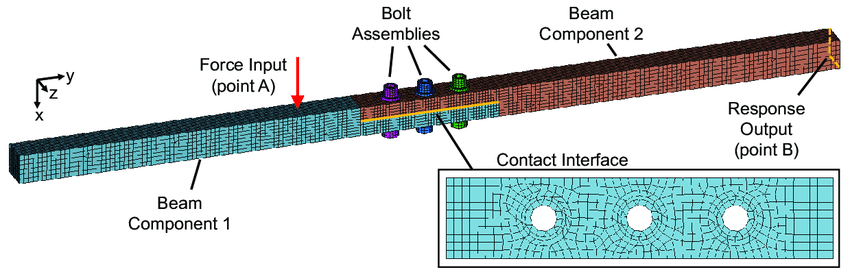
\includegraphics[width=\linewidth]{FIGS/brb}};

    \draw[red, very thick, rounded corners=0.5mm, fill=white, fill opacity=0.9,
    visible on=<2->] (-0.4932, 2.4583) rectangle (6.1918, -3.0000);
    \node[visible on=<2->, text width=0.5\textwidth, align=center] at
    (2.6164, -0.1528) {\rtxt{\textbf{Common theme}}: $\tikzmarkin<3>{a1}\text{Linear
        subcomponents}\tikzmarkend{a1}$ joined through a
      $\tikzmarkin<5->{a3}\text{non-linear contact interface}\tikzmarkend{a3}$
      undergoing $\tikzmarkin<4>{a2}\text{small deformation vibrations}\tikzmarkend{a2}$};

    \node[visible on=<3>, nidbox, text width=0.5\textwidth] at
    (2.5479, -2.8194) {\textbf{The HCB/CMS Methodology}
      
      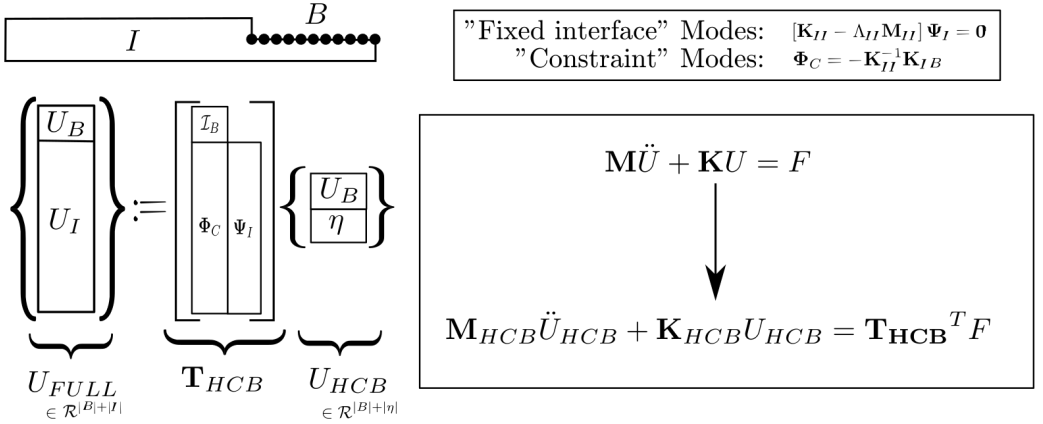
\includegraphics[width=\linewidth]{FIGS/hcb}
    };

    \node[visible on=<4>, nidbox, text width=0.5\textwidth] at
    (2.5479, -2.8194) {\textbf{Interface Virtual Element Representations}
      
      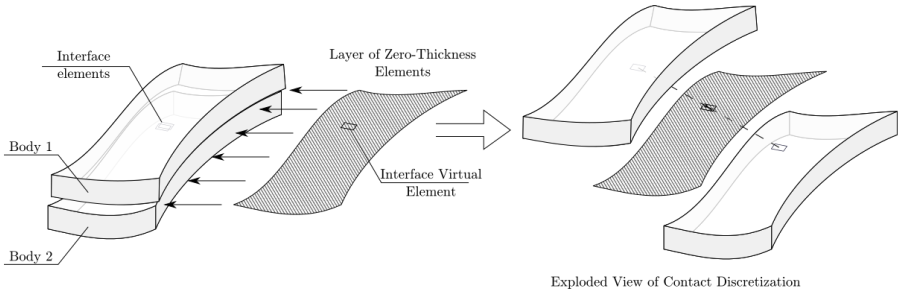
\includegraphics[width=\linewidth]{FIGS/ive}
    };

    \node[visible on=<5->, nidbox, text width=0.5\textwidth] at
    (2.5479, -2.8194) {\textbf{Interface Constitutive Modeling}
      
      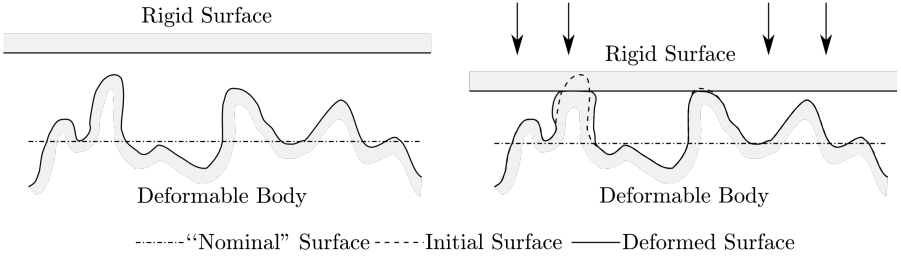
\includegraphics[width=\linewidth]{FIGS/roughc}
    };
  
    \node[visible on=<5->, text width=0.2\textwidth] at
    (-4.4383, -3.5833)
    {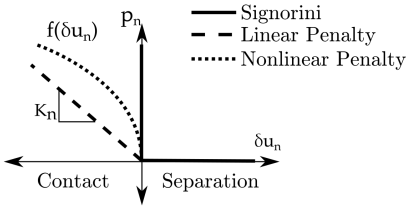
\includegraphics[width=\linewidth]{FIGS/normc}};
    \node[visible on=<5->, text width=0.2\textwidth] at
    (-2.0684, -2.9723)
    {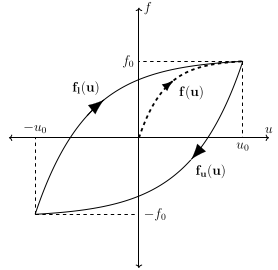
\includegraphics[width=\linewidth]{FIGS/tangc}};
    \node[visible on=<5->, text width=0.135\textwidth] at
    (-3.7260, -2.1944)
    {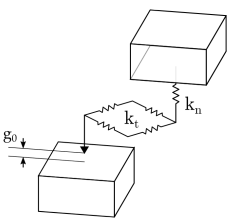
\includegraphics[width=\linewidth]{FIGS/contel}};      

    \node[visible on=<6->, nidbox, text width=0.43\textwidth] at
    (-3.3699, 0.4027) {\textbf{Nonlinear Responses}

      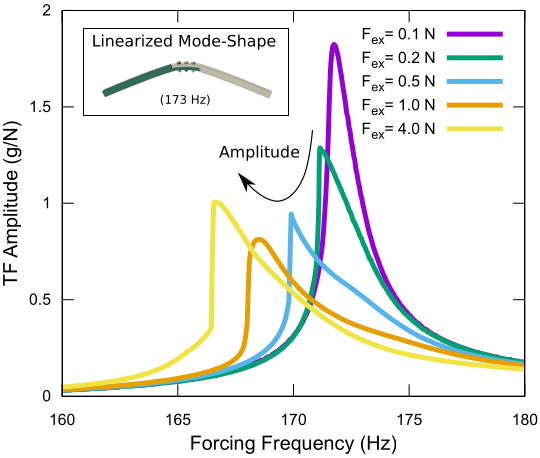
\includegraphics[width=0.8\linewidth]{FIGS/nlresp}
    };

    \node[visible on=<7->, nidbox, very thick, text
    width=0.6\textwidth] at (2.2877, 2.0556) {\rtxt{\textbf{Goal}}: Off-Load
      as much as possible to \textbf{focus on joints}.};
  \end{tikzpicture}
\end{frame}

\section{Outline of the Steps}
\label{sec:outline-steps}

\begin{frame}[label=cur]
  \frametitle{An Overview of the Modeling Pipeline}
  \framesubtitle{\insertsectionnumber.\insertsection}
  
\end{frame}


\section{Outro}
\label{sec:outro}

\begin{frame}
  \frametitle{\insertsectionnumber.~\insertsection}
  \begin{block}{\centering Acknowledgements}
    \begin{itemize}
    \item Prof. Matthew Brake
    \item Dr. Justin Porter, Maeve Karpov
    \item Prof. Matt Allen
    \end{itemize}
  \end{block}
\end{frame}

\begin{frame}[allowframebreaks]
  \frametitle{References}
  \renewcommand*{\bibfont}{\tiny}
  \vspace{-0.25cm}
  \printbibliography
\end{frame}

\end{document}

%%% Local Variables:
%%% mode: LaTeX
%%% TeX-master: t
%%% End:
